% This is samplepaper.tex, a sample chapter demonstrating the
% LLNCS macro package for Springer Computer Science proceedings;
% Version 2.21 of 2022/01/12
%
\documentclass[runningheads]{llncs}
%
\usepackage[T1]{fontenc}
% T1 fonts will be used to generate the final print and online PDFs,
% so please use T1 fonts in your manuscript whenever possible.
% Other font encondings may result in incorrect characters.
%
\usepackage{graphicx}
% Used for displaying a sample figure. If possible, figure files should
% be included in EPS format.
%
% If you use the hyperref package, please uncomment the following two lines
% to display URLs in blue roman font according to Springer's eBook style:
%\usepackage{color}
%\renewcommand\UrlFont{\color{blue}\rmfamily}
%
\usepackage{algorithmicx}
\usepackage{algorithm}
\usepackage{algpseudocode}
\usepackage{amsfonts}
\usepackage{amsmath}

\begin{document}
%
\title{Modeling graphene extraction process using generative diffusion models\thanks{Supported by Vilnius University.}}
%
\titlerunning{Modeling graphene extraction process using generative diffusion models}
% If the paper title is too long for the running head, you can set
% an abbreviated paper title here
%
\author{Modestas Grazys}%\inst{1}%\orcidID{0000-1111-2222-3333}}
%
\authorrunning{M. Grazys.}
% First names are abbreviated in the running head.
% If there are more than two authors, 'et al.' is used.
%
\institute{Institute of Computer Science\\ Vilnius University\\ Didlaukis st. 47 LT-08303, Vilnius, Lithuania\\ \email{modestas.grazys@mif.stud.vu.lt}\\}
%\url{https://mif.vu.lt/}\\}
%
\maketitle              % typeset the header of the contribution
%
\begin{abstract}
Graphene, a two-dimensional material composed of carbon
atoms arranged in a hexagonal lattice, possess a unique array of properties that make it a highly sought-after material for a wide range of applications. Its extraction process, a chemical reaction’s result, is represented as an image that shows areas of the synthesized material. Knowing the initial conditions (oxidizer) the synthesis result could be modeled by generating possible visual outcomes. A novel text2image pipeline to generate experimental images from chemical oxidizers is proposed. Key components of a such pipeline are a textual input encoder and a conditional generative model. In this work, the capabilities of certain text model and generative diffusion model are investigated and some conclusions are drawn providing further suggestions for further full text2image pipeline development\end{abstract}
%
%
%
\section{Introduction}
Graphene is an exotic wonder material with many advantages. It is the thinnest and strongest measured material in the universe. Graphene can maintain $10^{6}$ times higher current density than copper, has record thermal conductivity and stiffness, is impermeable to gases, and combines contradictory properties such as brittleness and ductility \cite{GrapheneDefinition}. It is a one-atom-thick material - a plane made up of carbon atoms lined up in a hexagonal lattice, resembling a beehive. Graphene has a very wide range of applications: manufacture of transistors \cite{GrapheneUseCases}; production of conductive plates with single-electron-transistor (SET) circuitry; digital memory for quantum repeaters \cite{GrapheneQuatumComputing}; plasma displays \cite{GraphenePlasmaDisplays} and much more.
\par
Graphene could be synthesized using methods described in \cite{GrapheneSynthesisVU,GICSynthesisVU}.
Yet, the development of a digital tool capable of visualizing the potential output of a graphene synthesis reaction using a selected oxidant could give an insight into the expected result beforehand. Instead of complex chemical process modeling, a such process could be modeled by analyzing images. The mathematical model for image encoding in our case is a neural network, which uses the process of automatic conversion of text into an image (\textit{text2image} \cite{text2image}), like Stable Diffusion or DALL-E 2 \cite{LatentDiffusion,DALLE}. Model input - chemical name (text) of the oxidant used in graphene synthesis. Then the output of the model - a visual representation (picture) of the result of a possible reaction. However, this will be discussed in more detail in a later work, in the future. And in the current context, more attention is paid to the separate components of the model architecture: the component that prepares the input text embeddings that condition the output and the generative component that provides the visual result of the synthesis simulation (diffusion model selected).
\par
For the component which prepares the input text embeddings (text encoder) the Contrastive Language-Image Pre-training model (CLIP) was selected \cite{CLIP}. The CLIP model can be conceptualized as a conventional image classifier with the ability to learn from the natural textual description of a photo. The usage of this model does not need complex and limiting data labeling methodologies. Also, the CLIP model can extract latent text embeddings, which can later influence the generative diffusion model in the process of conditional image generation. The simulation tool for the graphene synthesis reaction described in this paper specifically requires the text encoder component of the CLIP model for the latent text representations (text embeddings), precisely because of the influence on the diffusion model. The challenge here is to adapt appropriately this model to classify images of graphene synthesis correctly. As the images among oxidant classes look similar and the amount of data available is very limiting currently, because a larger amount of samples was not generated from the initial small dataset, provided by scientists working on graphene synthesis.
\par
For the generative component a diffusion model \cite{Diffusion,Diffusion_Ho} was selected. In this context, it is a generative neural network, like generative adversarial networks (\textit{GANs}) \cite{GAN} or variational autoencoders (\textit{VAEs}) \cite{VAE} capable of generating images from the input vector by applying a denoising process. The text latents encoded by the CLIP text encoder can influence the input vector of the diffusion model, thus conditioning the output of the diffusion model. In this way, potential imaging results of the graphene synthesis reaction can be generated conditioned by the entered name of the oxidant. However, this paper presents the capabilities of the diffusion model to generate imaging results for the graphene synthesis reaction by discarding this conditional input application and leaving this task for the future. The challenge here is to inspect the capability of a diffuser to generate graphene synthesis images and draw further conclusions about the usage of a conditional diffuser for the general development objective.
\par
The novelty of this work is the proposed usage of CLIP for digital components required for the subsequent modeling of the graphene synthesis simulation tool. This proposed solution allows the creation of a digital tool that can visually represent the possible output of the graphene synthesis reaction using the chosen oxidant. The tasks of the work include investigating the applicability of the CLIP model, the training process, and the ability of the diffusion-based generator (diffuser) to unconditionally generate images matching graphene synthesis reaction results.

\section{Methodology}

\subsection{Overview}

This text discusses digital tools that will be used to visualize the potential outcome of a graphene synthesis reaction using a selected oxidant. The two main tools used in this methodology are CLIP (Contrastive Language-Image Pre-training) and diffusion models. The CLIP model is used for image classification, learning to predict which oxidant corresponds to which image showing the result of a graphene synthesis reaction using an indicated oxidant. The CLIP text encoder can extract latent text embeddings from oxidant names. Text embeddings can then influence the input vectors of the diffusion model and thus condition the model output. Diffusion models, on the other hand, are used to create flexible and easily controlled generative models by systematically and slowly destroying image structure through an iterative diffusion process and learning the distribution of the added noise to reconstruct the image from the noise at inference. This section provides a brief summary of CLIP and diffusion model training and inference, including pseudocodes for the training and inference algorithms. The article concludes by highlighting the advantages of using CLIP and diffusion models in this context.

\subsection{CLIP}

The CLIP model \cite{CLIP} was introduced by the OpenAI company and is able to learn to predict which caption matches which image from the natural textual description of the photo. In this way, the limiting usability of computer vision systems is avoided, since conventional systems of this type require additional labeling information for any other visual concept. In implemented experimentation, the CLIP model is trained by providing (photo, text) data pairs, where text corresponds to the oxidant which was used to synthesize the result seen in the given photo. Conventional image classifiers simultaneously train a visual feature extractor and a linear classifier to predict the class label, while the CLIP model simultaneously trains a visual feature encoder and a text encoder to predict suitable (photo, text) pairs. Encoded oxidizer namings (latents) during training are encouraged to match synthesis result image latents as much as possible by minimizing pairs of their dot products. The minimized values are located on the main diagonal of this resulting matrix. The used architecture in our experimentation can be seen in Fig.~\ref{img:clip_traning}.
\par
\begin{figure}[h]
    \centering
    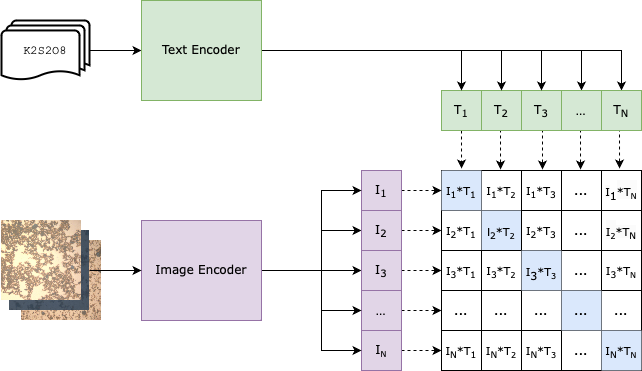
\includegraphics[scale=0.5]{img/CLIP_training.png}
    \caption{CLIP training} 
    \label{img:clip_traning}
\end{figure}
\par
During inference, the text encoder simulates a zero-shot linear classifier by embedding the oxidizer class names of the graphene images dataset and classifies the graphene synthesis results by their corresponding oxidizers. The image latent vector is scalar multiplied with each of the possible naming latent vectors and the smallest value of all obtained is selected. Then an oxidizer naming, which latent vector provided this smallest value in product with image latent, is selected and passed as an output. This process is illustrated by Fig.~\ref{img:clip_inference}.
\par
\begin{figure}[h]
    \centering
    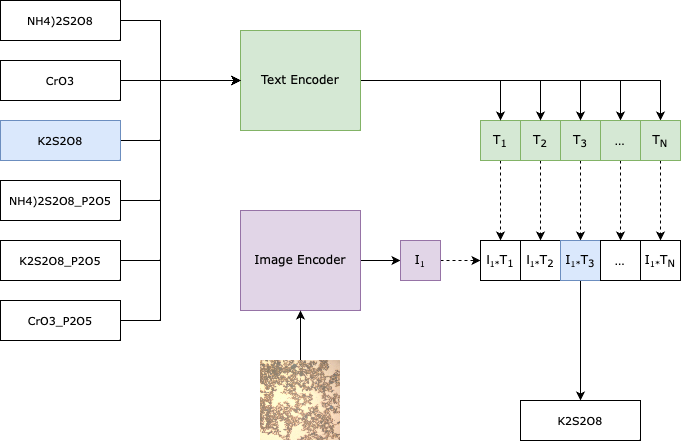
\includegraphics[scale=0.5]{img/CLIP_inference.png}
    \caption{CLIP inference}   % Antraštė įterpiama po paveikslėlio
    \label{img:clip_inference}
\end{figure}

Due to the property of learning from the natural textual description of an image, the CLIP model requires fewer data to achieve the same accuracy result compared to conventional computer vision classification models. These require a larger volume of training material corresponding to the distribution of use. This is relevant as the available amount of graphene data is very limited.
\par
The CLIP model with its ability to embed textual input is also used in models for generating images from a text: DALL-E 2, Stable Diffusion \cite{DALLE,LatentDiffusion}. It is this use case that is relevant to the purpose of this paper. Other use cases of the CLIP model: content moderation \cite{ContentModeration}; image captioning \cite{ImageCaptioning}; image search engine \cite{ImageSearch}; and much more.

\subsection{Diffusion model}

The invention of the diffusion model was inspired by the idea of non-equilibrium thermodynamics: to systematically and slowly destroy the data structure through an iterative process of diffusion. The reverse diffusion process can then be learned by reconstructing the previously destroyed data structure - this method creates an extremely flexible and easy-to-manage generative model \cite{Diffusion}.
\par
The diffusion process (forward process) is a Markov chain \cite{MarkovChains} and is performed by gradually adding Gaussian noise to the image data based on the noise variance schedule (\textit{variance schedule}) $\beta_1 , \beta_2, ..., \beta_T$, where T is the duration of the schedule (how many times noise will be added to the data). Fig.~\ref{img:diffusion_process} diffusion process is marked $q(x_t|x_{t-1})$, where $x_0 \sim q(x_0)$ - initial data; $x_1, x_2, ..., x_{t-1}, x_t, ..., x_T$ - latents (data with applied Gaussian noise). \\
\begin{figure}[H]
    \centering
    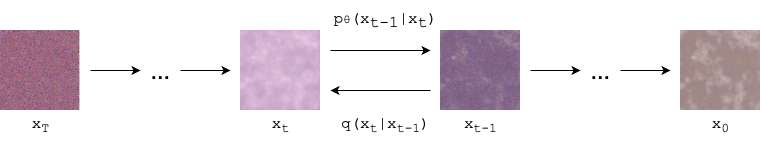
\includegraphics[scale=0.45]{img/Markov_Chain.png}
    \caption{Diffusion process - Markov chain}
    \label{img:diffusion_process}
\end{figure}
Mathematically, the diffusion process $q(x_{1:T}|x_0)$ is written \cite{Diffusion_Ho}:
\begin{equation}
q(x_{1:T}|x_0) := \prod_{t=1}^{T}q(x_t|x_{t-1}), \quad\quad q(x_t|x_{t-1}) := \mathcal{N}(x_t| \sqrt{1 - \beta_t}x_{t-1}, \beta_t\textbf{I}) \label{eq:diffusion_process}
\end{equation}

The reverse process Fig.~\ref{img:diffusion_process} is denoted by $p_\theta(x_{t-1}|x_t)$. Is run to reconstruct image data destroyed by noise and is described by a Markov chain with learned Gaussian transitions starting from $p(x_T) = \mathcal{N}(x_T| \textbf{0}, \textbf{I}):$
\begin{equation}
p_\theta(x_{0:T}) := p(x_T)\prod_{t=1}^{T}p_\theta(x_{t-1}|x_t), \quad\quad p_\theta(x_{t-1}|x_t) := \mathcal{N}(x_{t-1}| \boldsymbol{\mu}_\theta(x_t, t), \boldsymbol{\Sigma}_\theta(x_t, t))
\label{eq:reverse_process}
\end{equation}
We can write a closed-form expression for the loss function \cite{Diffusion_Ho,Diffwave}:
\begin{equation}
L = c + \sum_{t=1}^T\kappa_t\mathbb{E}_{x_0,\epsilon}\Big|\Big|\epsilon - \epsilon_\theta(\sqrt{\prod_{s=1}^t(1 - \beta_t)} \cdot x_0 + \sqrt{1 - \prod_{s=1}^t(1 - \beta_t)} \cdot \epsilon, t)\Big|\Big|_2^2
\label{eq:loss_calculation_closed}
\end{equation}
Here, $c$ and $\kappa_t$ are constants independent of $\theta$. $\kappa_t = \frac{\beta_t}{2(1 - \beta_t)(1 - \prod_{s=1}^t(1 - \beta_{t-1}))}$ when $t > 1$, but $\kappa_1 = \frac{1} {2(1 - \beta_1)}$. Also, $\epsilon_\theta:\mathbb{R}^L \times \mathbb{N} \rightarrow \mathbb{R}^L$ is a neural network that takes a latent variable $x_t$ and a diffusion step $t$ as the input
\\ \\
Below are the pseudocodes for the diffusion model training and inference (sampling) algorithms based on all the above information.
\\
\begin{minipage}{0.47\textwidth}
    \begin{algorithm}[H]
        \caption{Training}
        \begin{algorithmic}
            \Repeat
                \State $x_0 \sim q(x_0)$
                \State $t \sim Uniform(\left\{1, ..., T\right\})$
                \State $\epsilon \sim \mathcal{N}(\bold{0}, \bold{I})$
                \State Gradient descent step: 
                \State \quad$\nabla_\theta\Big|\Big|(\epsilon - \epsilon_\theta(\sqrt{\prod_{s=1}^t(1 - \beta_t)} \cdot x_0 + \sqrt{1 - \prod_{s=1}^t(1 - \beta_t)} \cdot \epsilon, t)\Big|\Big|^2$
            \Until converged
        \end{algorithmic}
    \end{algorithm}
\end{minipage}
\hfill
\begin{minipage}{0.47\textwidth}
    \begin{algorithm}[H]
        \caption{Sampling}
        \begin{algorithmic}
            \vspace{7pt}
            \State $x_T \sim \mathcal{N}(\bold{0}, \bold{I})$
            \For{$t=T,...,1$}
                \State $z \sim \mathcal{N}(\bold{0}, \bold{I})$ if $t > 1$, else $z = \bold{0}$
                \State $x_{t-1} = \frac{1}{\sqrt{(1 - \beta_t)}}(x_t - \frac{\beta_t}{\sqrt{1 - \prod_{s=1}^t(1 - \beta_t)}}\epsilon_\theta(x_t, t)) + \sigma_tz$
            \EndFor \\
            \Return $x_0$
            \vspace{10pt}
        \end{algorithmic}
    \end{algorithm}
\end{minipage}
\\
\\
During inference, a noise latent is passed through the diffuser and an image representing a graphene synthesis result is expected to appear.
\par
To solve this work's tasks, it is enough to realize that the diffusion model can generate images of possible graphene synthesis results, so this model was chosen for this very reason. Using the cross-attention layers in the model architecture can influence the model's generative processes, thus, through the input, conditioning the model's output. And this is relevant to the general goal of the work, which will be worked on in the future. This work is limited to research to determine the capabilities of the diffusion model to unconditionally generate images of possible graphene synthesis results.

\begin{figure}[h]
    \centering
    \includegraphics[scale=0.13]{img/examples-2.png}
    \caption{Optical microscopy samples of graphite bisulfate (GBS)}
\end{figure}

\section{Computational experiments}

All studies were performed in the Google Colab Premium environment using A100 SXM4 40GB GPU.

\subsection{Data}

Before conducting the research, 79 images of graphene synthesis results (optical microscopy photographs of graphite bisulfate (GBS) samples) with specified oxidants and reagents, which were used during the synthesis, were obtained from the Faculty of Chemistry and Geosciences of Vilnius University. In GBS synthesis, three different oxidants were used:
\begin{itemize}
    \item Ammonium persulfate - $(NH_4)_2S_2O_8$
    \item Potassium persulfate - $K_2S_2O_8$
    \item Chromium trioxide - $CrO_3$
\end{itemize}
The GBS synthesis procedure was repeated using all the oxidants and additionally adding a water binding reagent - phosphorus pentoxide $P_2O_5$ to the oxidizing mixture. Thus, a total of six data classes were obtained, which are named:\\
\begin{itemize}
    \item NH4)2S2O8
    \item K2S2O8
    \item CrO3
    \item NH4)2S2O8\_P2O5
    \item K2S2O8\_P2O5
    \item CrO3\_P2O5
\end{itemize}

\subsection{Data processing}

The raw data are JPG format photos with a resolution of 2560 x 1920. The pictures show the result on a large scale, but the number of pictures is not large, so for a better quality of network generalization, a 1000 x 1000 resolution frame is selected at a random place in the picture and the picture is cropped around the frame. However, the resolution of a 1000 x 1000 photo is extremely high and its processing would theoretically require a very large neural network, the calculations of which would be extremely expensive, so the resolution of the photo is reduced to 128 x 128. These augmentations are chosen for optimal model training and subsequent exploitation without damaging essential information in the data.

\subsection{CLIP model training}

The individual components that make up the CLIP model were downloaded using the Hugging Face \texttt{transformers} library \cite{wolf-etal-2020-transformers}: the CLIP photo encoder component and the CLIP text encoder component. This decomposition is chosen for convenience in the later implementation of the overall goal of the work, which requires only the CLIP text encoder component. Also downloaded: CLIP feature extractor and CLIP tokenizer in \texttt{"openai/clip-vit-base-patch32"} configuration. Settings for the CLIP video encoder and text input encoder components can be found in appendix \ref{app:clip hyperparameters}. Projection heads of photo embeddings and text embeddings were also used, which unify the dimensions of the embeddings. These heads are small neural networks consisting of one residual block \cite{ResNet}, the diagram is presented in appendix \ref{app:projection_head}.
\\\par
The CLIP model was trained by providing it with (picture, text) data pairs:\\
\\
\begin{minipage}{0.47\textwidth}
    \begin{enumerate}
        \item The photo is passed through the CLIP image feature extractor
        \item The resulting processed photo is passed through the CLIP image encoder
        \item The resulting latents are passed through the projection head
    \end{enumerate}
\end{minipage}
\hfill
\begin{minipage}{0.47\textwidth}
    \begin{enumerate}
        \item The text is passed through the CLIP tokenizer.
        \item The resulting tokens are passed through the CLIP text encoder
        \item The resulting latents are passed through the projection head
    \end{enumerate}
\end{minipage}
\vspace{0.5cm} \\
Later, the probabilities are calculated, the value of the cross entropy loss function is estimated, the gradient is calculated and the CLIP components' weights are updated. For the training process an Adam optimizer \cite{Adam} and a cosine learning rate scheduler \cite{CosineScheduler} were used. It was performed using the Hugging Face \texttt{accelerate} library for training over 200 epochs \cite{accelerate}.

\subsection{Diffusion model training}

The diffusion model was downloaded from the Hugging Face \texttt{diffusers} library \cite{von-platen-etal-2022-diffusers}. Unet architecture for this model was used. A scheme describing the model architecture is given in appendix \ref{app:diffuser_scheme}. Settings and hyperparameters are given in appendix \ref{app:diffuser_config}. Also, from the \texttt{diffusers} library a \texttt{DDPM} noise scheduler according to \cite{Diffusion_Ho} was downloaded.
\par
The diffusion model was trained by loading batches of pictures to it:
\begin{enumerate}
    \item Noise is added to photos according to the noise schedule
    \item Noisy pictures are passed through a diffusion model
    \item The obtained noise estimate of the model is evaluated with the noise schedule reference and the value of the mean square error (MSE) loss function is calculated
    \item Based on the received value, the gradient is calculated and the model weights are updated
\end{enumerate}
For training, over 200 epochs, the Adam optimizer \cite{Adam} with decoupled weight loss regularization \cite{AdamW}, the cosine learning rate scheduler \cite{CosineScheduler} were used, and the training process was performed using the Hugging Face \texttt{accelerate} library \cite{accelerate}. Afterward, the diffuser images were generated using the \texttt{DDPMPipeline} class from the \texttt{diffusers} library. The implementation code will be shared in the future.

\section{Results}

\subsection{CLIP results}

For this work, CLIP model inference provided disappointing results. Currently, the model is not able to reliably classify the imaging data of graphene synthesis - for each of the classes of oxidants with which graphene was synthesized, the model assigns approximately equal probabilities during classification, trying to guess the real oxidant.
\\
\begin{minipage}{0.5\textwidth}
    \begin{table}[H]
        \centering
        \caption{CLIP inference 1}
        {\begin{tabular}{|l|c|c|} 
            \hline
            Top predictions & \\
            \hline
            NH4)2S2O8\_P2O5 & 16.76\% \\
            \hline
            NH4)2S2O8 & 16.71\% \\
            \hline
            K2S2O8\_P2O5 & 16.67\% \\
            \hline
            Actual text prompt & NH4)2S2O8\_P2O5 \\
            \hline
        \end{tabular}}
        \label{tab:clip_inference_example_1}
    \end{table}
\end{minipage}
\hfill
\begin{minipage}{0.5\textwidth}
    \begin{table}[H]
        \centering
        \caption{CLIP inference 2}
        {\begin{tabular}{|l|c|c|} 
            \hline
            Top predictions & \\
            \hline
            CrO3 & 16.78\% \\
            \hline
            K2S2O8 & 16.74\% \\
            \hline
            CrO3\_P2O5 & 16.72\% \\
            \hline
            Actual text prompt & NH4)2S2O8 \\
            \hline
        \end{tabular}}
        \label{tab:clip_inference_example_2}
    \end{table}
\end{minipage}
\hfill
\begin{minipage}{1.0\textwidth}
    \begin{table}[H]
        \centering
        \caption{CLIP inference 3}
        {\begin{tabular}{|l|c|c|} 
            \hline
            Top predictions & \\
            \hline
            NH4)2S2O8\_P2O5 & 16.73\% \\
            \hline
            NH4)2S2O8 & 16.70\% \\
            \hline
            K2S2O8\_P2O5 & 16.67\% \\
            \hline
            Actual text prompt & NH4)2S2O8 \\
            \hline
        \end{tabular}}
        \label{tab:clip_inference_example_3}
    \end{table}
\end{minipage}
\vspace{0.5cm} \\
The figures above show three attempts to determine the oxidant, used to synthesize graphene, from a photograph. The "\textit{Actual text prompt}" box in the tables shows the actual graphene synthesis result class, and above it, in descending order, the class predictions with probabilities. From the Table~\ref{tab:clip_inference_example_1} example, we can see that the model correctly identified the oxidant class, but the other guesses get slightly lower probabilities. Similar classification probabilities are also seen in the Table~\ref{tab:clip_inference_example_2}-\ref{tab:clip_inference_example_3} examples, where the model failed to correctly identify the graphene synthesis oxidant, and Table~\ref{tab:clip_inference_example_2} the correct oxidizer class is not even among the three most likely guesses. It is believed that in this design, the CLIP model fails to draw strong differences between graphene synthesis samples synthesized with different oxidants, and in the latent space, all latents: both text and photos, are too closely spaced.

\subsection{Diffusion model results}

A mathematical expression for evaluating the quality of the model, except for the loss function, was not designed, therefore the most optimal hyperparameter values were selected by comparing the values of the loss function calculated after the appropriate number of training epochs. Forty (40) training epochs were found to suit the need for training the generative diffuser, as the following number of them did not make significant learning progress. It was found that the most optimal tested learning rate value for this model is equal to $3 * 10^{-4}$. With values of this hyperparameter higher than $10^{-3}$, the model diverged. The study results are provided in Fig.~\ref{img:learning_rate_results}.
\\
\begin{minipage}{0.47\textwidth}
    \begin{figure}[H]
        \centering
        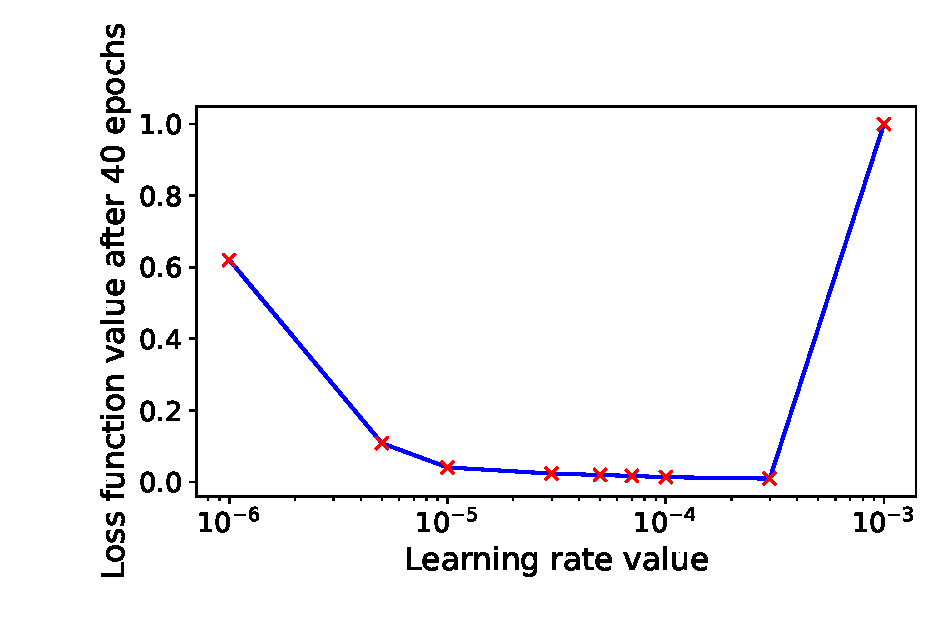
\includegraphics[scale=0.36]{img/learning_rate.eps}
        \caption{Learning rate study for the diffuser}
        \label{img:learning_rate_results}
    \end{figure}
\end{minipage}
\hfill
\begin{minipage}{0.47\textwidth}
    \begin{figure}[H]
        \centering
        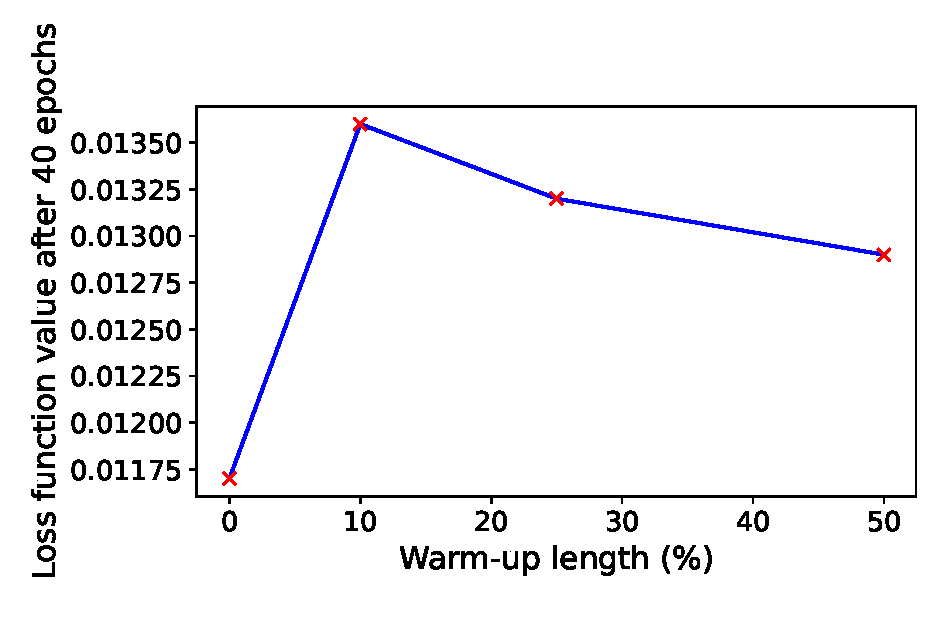
\includegraphics[scale=0.36]{img/warm_up.eps}
        \caption{Learning rate scheduler warm up study for the diffuser}
        \label{img:cosine_warmup_results}
    \end{figure}
\end{minipage}
\vspace{0.5cm} \\
The warm-up \cite{CosineScheduler} of the cosine training step planner was also investigated. Warm-up values of different lengths were tested as a percentage (\%) of the number of warm-up steps from the total number of model training steps. The optimal value of this hyperparameter was found to be 0\%. A warm-up study of the cosine training step scheduler is displayed in Fig.~\ref{img:cosine_warmup_results}.
\par
The results of diffusion model generation were evaluated visually and by Frechet Inception Distance (FID) metric \cite{fid}. The images generated unconditionally by the model look similar to the images that were fed to the model during training. However, a closer look at the results reveals a lack of detail clarity - it is difficult to accurately distinguish graphene regions in generated images. This problem may be caused by the small amount of data and the low resolution of the generated photo (128 x 128). Examples of generated images are provided in Fig.~\ref{img:diffuser_inference_results}. \par
Frechet Inception Distance was calculated by comparing original photos (training data), disregarding the classes of the sample, with:
\begin{enumerate}
    \item The same sample of original data
    \item The same sample of original data, but within the same classes
    \item Random images
    \item Generated images by the first iteration model
    \item Generated images by the best model
\end{enumerate}
The results are shown in Fig.~\ref{img:fid_results} - original FID score values and Fig.~\ref{img:fid_results_percetages} - percentages of the scores compared with the highest score. The highest FID score, indicating the worst result, is reached by the first iteration's model-generated images. The best model's generated images reach 68.51\% of the highest score and indicate a better resemblance of the generated photos to the original than comparing original data with random images. Yet the score is far from the original data's comparison as it reaches negligible FID value and is the target of this task.
\\
\begin{minipage}{0.47\textwidth}
    \begin{figure}[H]
        \centering
        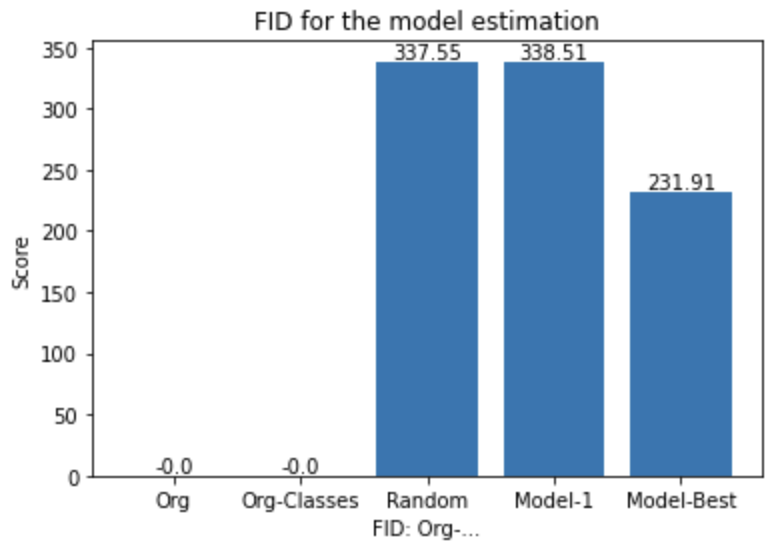
\includegraphics[scale=0.4]{img/FID_scores.png}
        \caption{Frechet Inception Distance scores}
        \label{img:fid_results}
    \end{figure}
\end{minipage}
\hfill
\begin{minipage}{0.47\textwidth}
    \begin{figure}[H]
        \centering
        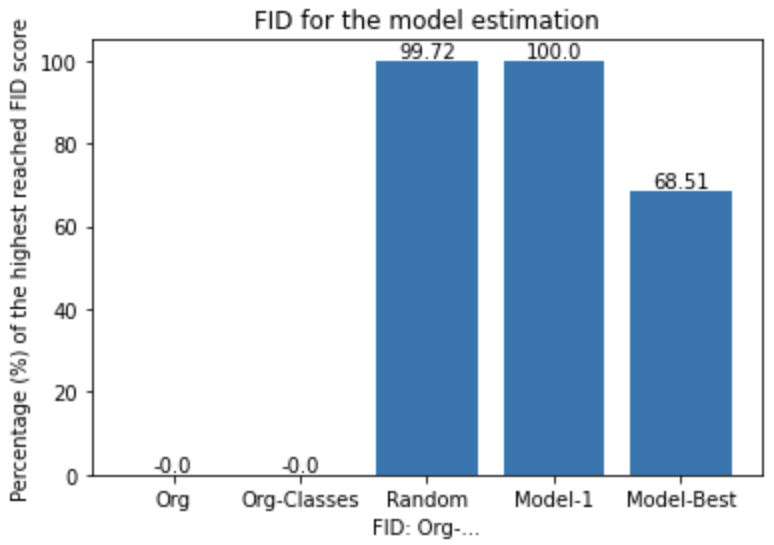
\includegraphics[scale=0.36]{img/FID_percentages.png}
        \caption{Frechet Inception Distance score percentages}
        \label{img:fid_results_percetages}
    \end{figure}
\end{minipage}
\\
\begin{figure}[h]
    \centering
    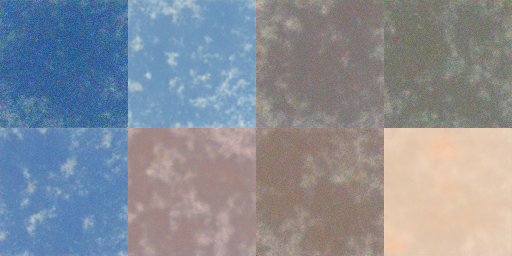
\includegraphics[scale=0.65]{img/graphene-diffuser-inference.png}
    \caption{Generated samples (resolution 128 x 128)}
    \label{img:diffuser_inference_results}
\end{figure}

\section*{Conclusion} % with asterisk (*) section becomes non-numerable

The novel text2image usage to encode chemical formulas for the generation of chemical images was proposed and successfully implemented. The results demonstrated the image generation part to be working more sufficiently than the graphene synthesis results classification. The encoder model assigns similar probabilities to all guess variants of the class. Furthermore, the diffusion model (generator) generates images similar to what would be expected, but these images are not detailed enough, lacking resolution. However, based on the tasks of text2image, these two models can be adapted to predict the results of graphene synthesis reactions.
\par
On the other hand, for the development of a high-quality image prediction tool, there remain a number of tasks related to the adaptation of the CLIP model and the generative diffuser.
%
% ---- Bibliography ----
%
% BibTeX users should specify bibliography style 'splncs04'.
% References will then be sorted and formatted in the correct style.
%
\bibliographystyle{splncs04}
\bibliography{bibliography}

\appendix

\section{The used CLIP model configuration}
\label{app:clip hyperparameters}
\subsection{CLIP image encoder configuration}

\begin{table}[H]\footnotesize
  \centering
  \caption{CLIP image encoder configuration}
  {\begin{tabular}{|l|c|c|} 
        \hline
        Hidden layers dimension (\textit{hidden\_size}) & 768 \\
        \hline
        Encoder's feed-forward layer dimension (\textit{intermediate\_size}) & 3072 \\
        \hline
        Number of hidden layers (\textit{num\_hidden\_layers}) & 12 \\
        \hline
        Number of attention heads (\textit{num\_attention\_heads}) & 12 \\
        \hline
        Number of image color channels (\textit{num\_channels}) & 3 \\
        \hline
        Resolution of images (\textit{image\_size}) & 128 x 128 \\
        \hline
        Resolution of an attention patch (\textit{patch\_size}) & 32 \\
        \hline
        Hidden layers' activation function (\textit{hidden\_act}) & "quick\_gelu" \\
        \hline
        Normalization layers' epsilon $\epsilon$ value (\textit{layer\_norm\_eps}) & 1e-05 \\
        \hline
        Dropout probability in fully connected layers
        (\textit{dropout}) & 0.0 \\
        \hline
        Dropout probability in attention layers (\textit{attention\_dropout}) & 0.0 \\
        \hline
        The standard deviation of model weights initiation
        (\textit{initializer\_range}) & 0.02 \\
        \hline
        Model weights initiation factor (\textit{initializer\_factor}) & 1.0 \\
        \hline
  \end{tabular}}
  \label{tab:CLIP vision model config}
\end{table}

\subsection{CLIP text encoder configuration}

\begin{table}[H]\footnotesize
  \centering
  \caption{CLIP text encoder configuration}
  {\begin{tabular}{|l|c|c|} 
        \hline
        Vocabulary size (\textit{vocab\_size}) & 49408 \\
        \hline
        Hidden layers dimension (\textit{hidden\_size}) & 512 \\
        \hline
        Encoder's feed-forward layer dimension (\textit{intermediate\_size}) & 2048 \\
        \hline
        Number of hidden layers (\textit{num\_hidden\_layers}) & 12 \\
        \hline
        Number of attention heads (\textit{num\_attention\_heads}) & 8 \\
        \hline
        The maximum tokenized sequence length (\textit{max\_position\_embeddings}) & 77 \\
        \hline
        Hidden layers' activation function (\textit{hidden\_act}) & "quick\_gelu" \\
        \hline
        Normalization layers' epsilon $\epsilon$ value (\textit{layer\_norm\_eps}) & 1e-05 \\
        \hline
        Dropout probability in fully connected layers (\textit{dropout}) & 0.0 \\
        \hline
        Dropout probability in attention layers (\textit{attention\_dropout}) & 0.0 \\
        \hline
        Standard deviation of model weights initiation (\textit{initializer\_range}) & 0.02 \\
        \hline
        Model weights initiation factor (\textit{initializer\_factor}) & 1.0 \\
        \hline
        The ID of the padding token (\textit{pad\_token\_id}) & 1 \\
        \hline
        The ID of the beginning-of-stream token (\textit{bos\_token\_id}) & 0 \\
        \hline
        The ID of the end-of-stream token (\textit{eos\_token\_id}) & 2 \\
        \hline
  \end{tabular}}
  \label{tab:CLIP text model config}
\end{table}

\subsection{General CLIP configuration and hyperparameters}

\begin{table}[H]\footnotesize
  \centering
  \caption{General CLIP configuration and hyperparameters}
  {\begin{tabular}{|l|c|c|} 
        \hline
        Training batch size & 26 \\
        \hline
        Number of training epochs & 200 \\
        \hline
        Gradient accumulation steps & 1 \\
        \hline
        Learning rate & $5 \cdot 10^{-2}$ \\
        \hline
        CLIP temperature & 0 \\
        \hline
        Learning rate warm-up steps & 0 \\
        \hline
        Latents dimension & 256 \\
        \hline
  \end{tabular}}
  \label{tab:CLIP hyperparameters}
\end{table}


\section{Embeddings projection head scheme}
\label{app:projection_head}

\begin{figure}[H]
    \centering
    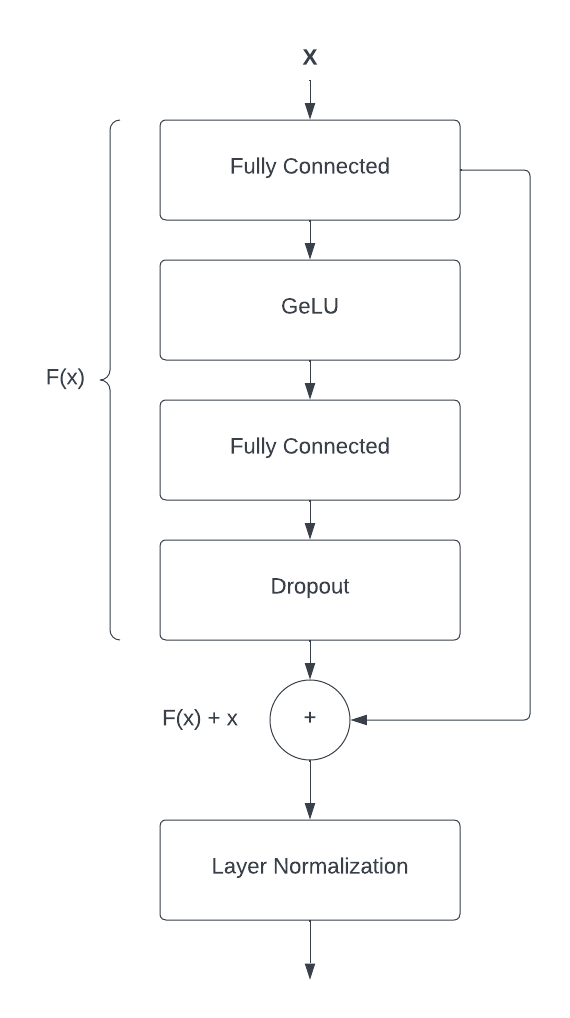
\includegraphics[scale=0.3]{img/Residual layer.png}
    \caption{Embeddings projection head scheme}   % Antraštė įterpiama po paveikslėlio
    \label{img:projection_head}
\end{figure}

\section{Diffusion model configuration and hyperparameters}
\label{app:diffuser_config}

\begin{table}[H]\footnotesize
  \centering
  \caption{Diffusion model configuration and hyperparameters}    % Antraštė įterpiama prieš lentelę
  {\begin{tabular}{|l|c|c|} 
        \hline
        Resolution of generated photos & 128 \\
        \hline
        Number of input image channels & 3 \\
        \hline
        Number of output image channels & 3 \\
        \hline
        Number of training epochs & 200 \\
        \hline
        Gradient accumulation steps & 1 \\
        \hline
        Learning rate & $3 \cdot 10^{-4}$ \\
        \hline
        Learning rate warm-up steps & 0 \\
        \hline
        Number of diffusion steps & 1000 \\
        \hline
  \end{tabular}}
  \label{tab:Diffuser hyperparameters}
\end{table}

\section{Architecture of the diffusion model - Unet}
\label{app:diffuser_scheme}

\begin{figure}[H]
    \centering
    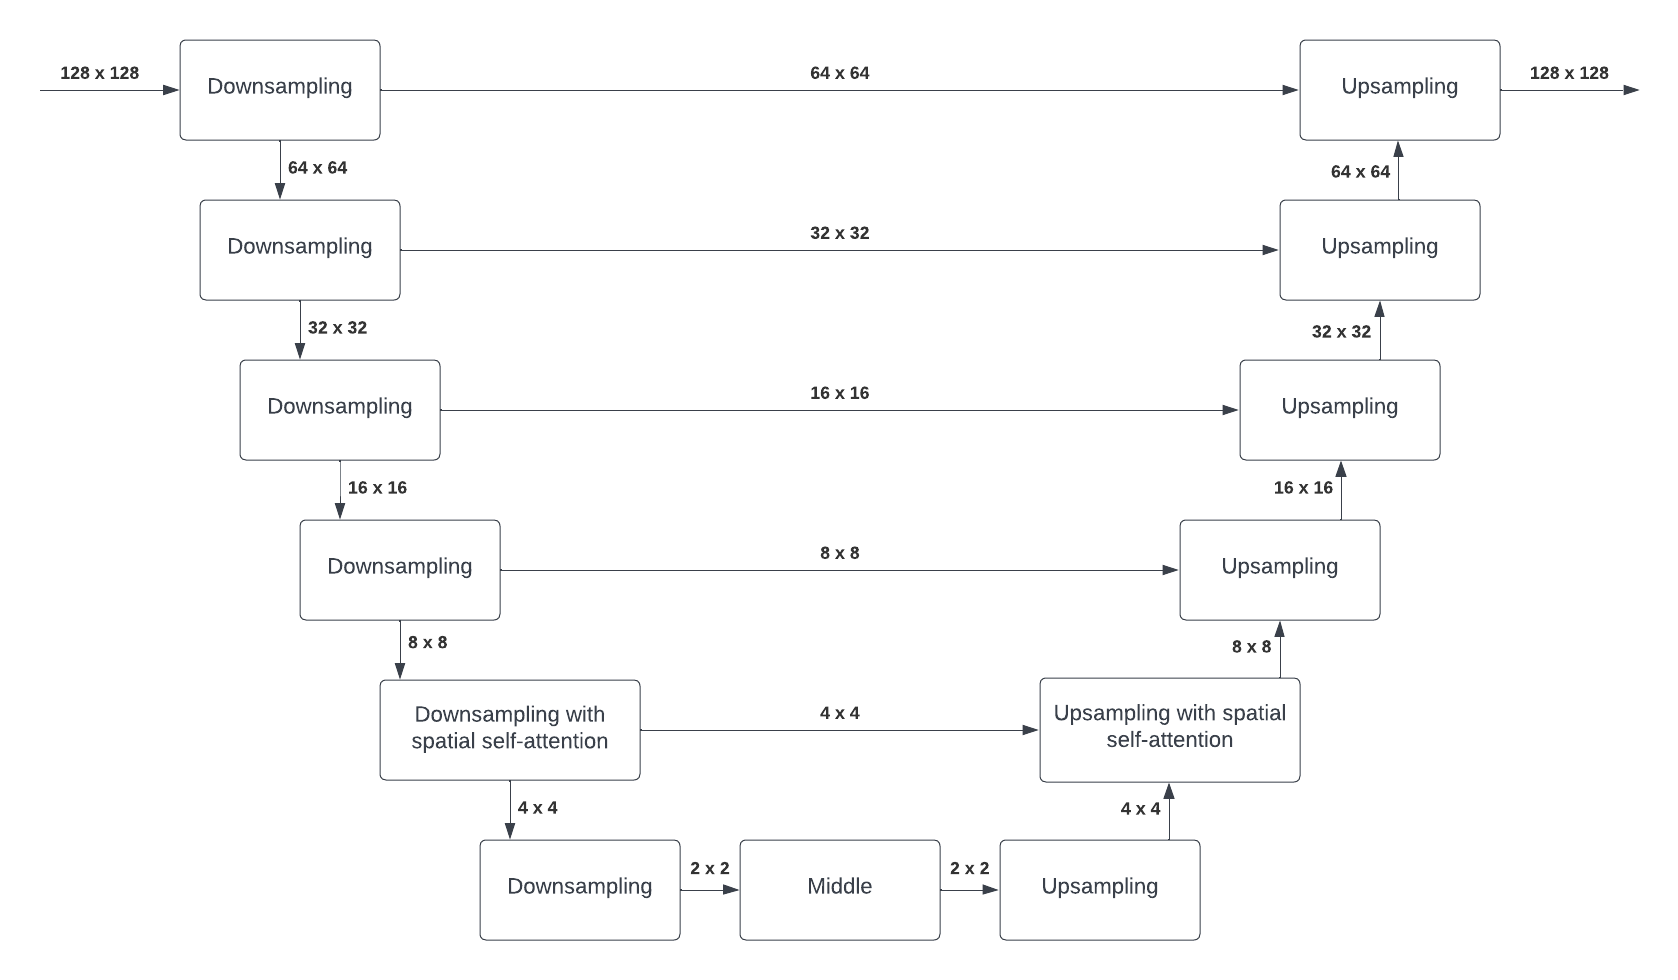
\includegraphics[scale=0.22]{img/Diffuser-unet.png}
    \caption{Architecture of the diffusion model - Unet}   % Antraštė įterpiama po paveikslėlio
    \label{img:diffuser_scheme}
\end{figure}

\end{document}
